\chapter{Bestimmung der Lasten nach CS 23}\label{cha:Bestimmung der Lasten nach CS 23}

\section{Ausgangsannahmen für das Fluggerät}

Das Fluggerät und der Tragflügel werden für die gegebene Flugaufgabe anhand folgender Parameter ausgelegt:

\begin{table}[h]
\centering
\begin{tabular}{|l|l|l|l|}
\hline
Parameter  & Bezeichnung &  Wert & Einheit \\ \hline
Fluggeschwindigkeit  & $V_{reise}$ & 15,0 & $m/s$\\ \hline
Abfluggewicht & $m_{reise}$  & 5,0 & $kg$\\ \hline
Profilierung & Clark-Y & - & - \\ \hline
Segmentteilung & $Y_{seg}$ & 700 & mm\\ \hline
\end{tabular}
\caption{Grundannahmen für das System}
\label{tab:Grundannahmen für das System}
\end{table}

\subsection{Sicherheiten und Anforderungen}

Bei der Berechnung der Lasten und der drauf aufbauenden Dimensionierung wird von den in Tabelle \ref{} im Anhang dargelegten Sicherheiten und Anforderungen an das Flugzeug  ausgegangen.

\subsection{Der Tragflügel}

Der Tragflügel wird für die gegebene Flugaufgabe anhand folgender Parameter ausgelegt:

\begin{figure}[H]
\centering
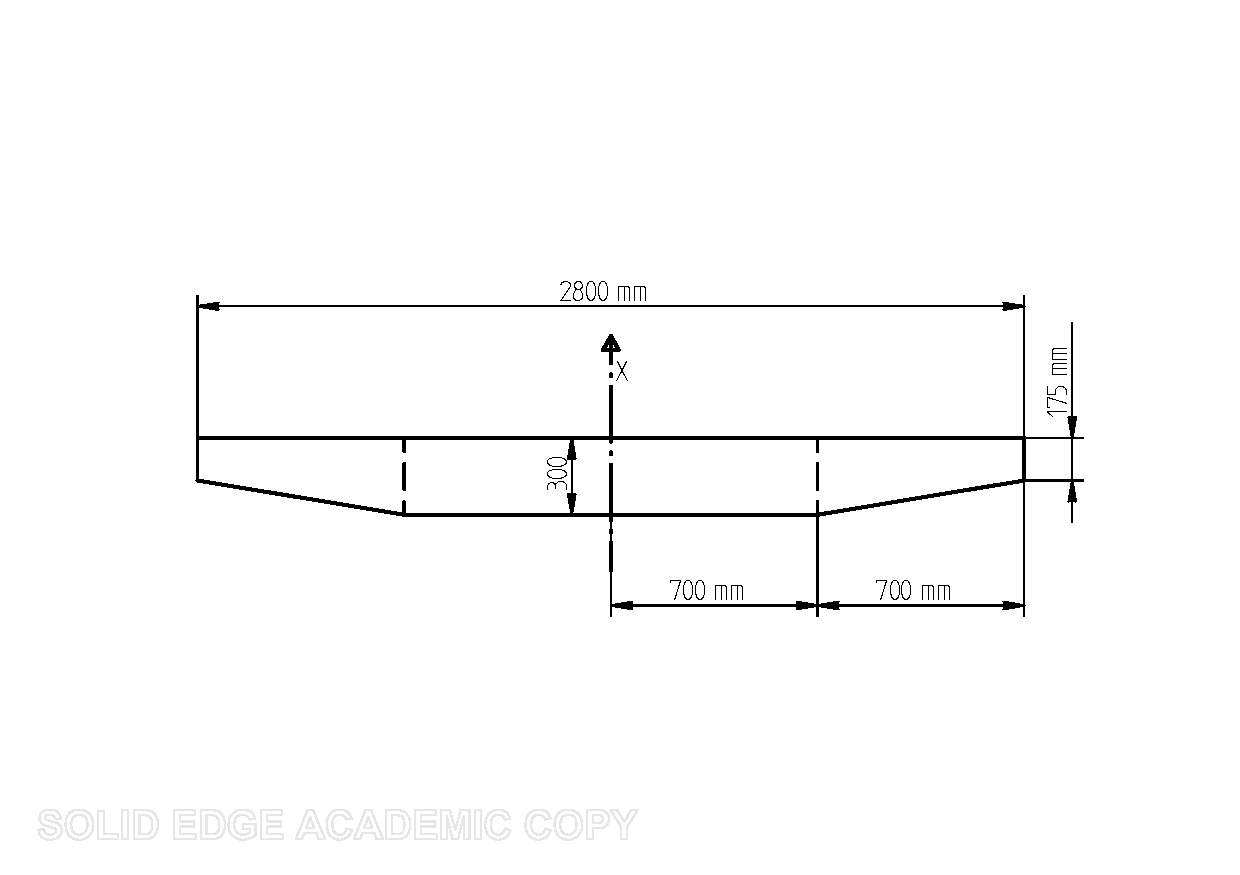
\includegraphics[width=0.9\textwidth, trim={15mm 40mm 15mm 40mm},clip]{bilder/Fotos/Grundriss_Flaeche.pdf}
\caption{Aufriss mit Eckdaten der Fläche} 
\label{fig:Flächenaufriss}
\end{figure}

Die Tragfläche setzt sich aus einem zentralen rechteckigen Segment und jeweils daran angeschlossenen Außensegmenten 
in Trapezform zusammen.
Hierbei werden Eigenschaften von bisher eingesetzten Flügeln übernommen.
Eine weitergehende Diskussion über die Wahl dieser aerodynamischen Parameter soll in dieser Arbeit nicht stattfinden. 
%\colorbox{red}{Es wird von der Strukturauslegung ausgegangen.}
Die Wahl von geradlinig aufgebauten Tragflächensegmenten ermöglicht hier Vorteile bei der Fertigung.\\
Im Bild \ref{fig:Flächenaufriss} ist ein Aufriss mit den Grundabmessungen dargestellt,welche für die aerodynamische Berechnung und den mechanischen Aufbau verwendet werden.

\begin{table}[h]
\centering
\begin{tabular}{|l|l|l|l|}
\hline
Parameter  & Bezeichnung &  Wert & Einheit \\ \hline
Spannweite  & $V_{reise}$ & 2800 & $mm$\\ \hline
Projizierte Fläche & $A_{ref}$  & 0,752 & $m^2$\\ \hline
Wurzeltiefe & $CH_{Wurzel}$ & 300 & $mm$ \\ \hline
Spitzenverwindung & $\alpha_{Spitze}$ & -\,2 & $^\circ$\\ \hline
Mittlere Flügeltiefe & $l_{\mu}$ & 275 & $mm$ \\ \hline
\end{tabular}
\caption{Dimensionen des Tragflügels}
\label{tab:Dimensionen des Tragflügels}
\end{table}

\clearpage


\section{Bestimmung der Lasten}
Mit einem Gewicht von 5,0 kg gehört das Fluggerät gemäß CS 23 der Kategorie \glqq Normal\grqq{} an.
Alle Auslegungsrechnungen beziehen sich auf diese Eingliederung.


\subsection{Lasten im stationären Flug}
Im Folgenden zeigt die Abbildung \ref{fig:Stationärer Reiseflug in XFLR} den aeroynamischen Entwurf im stationär ausgelegten Reiseflug.

\begin{figure}[H]
\centering
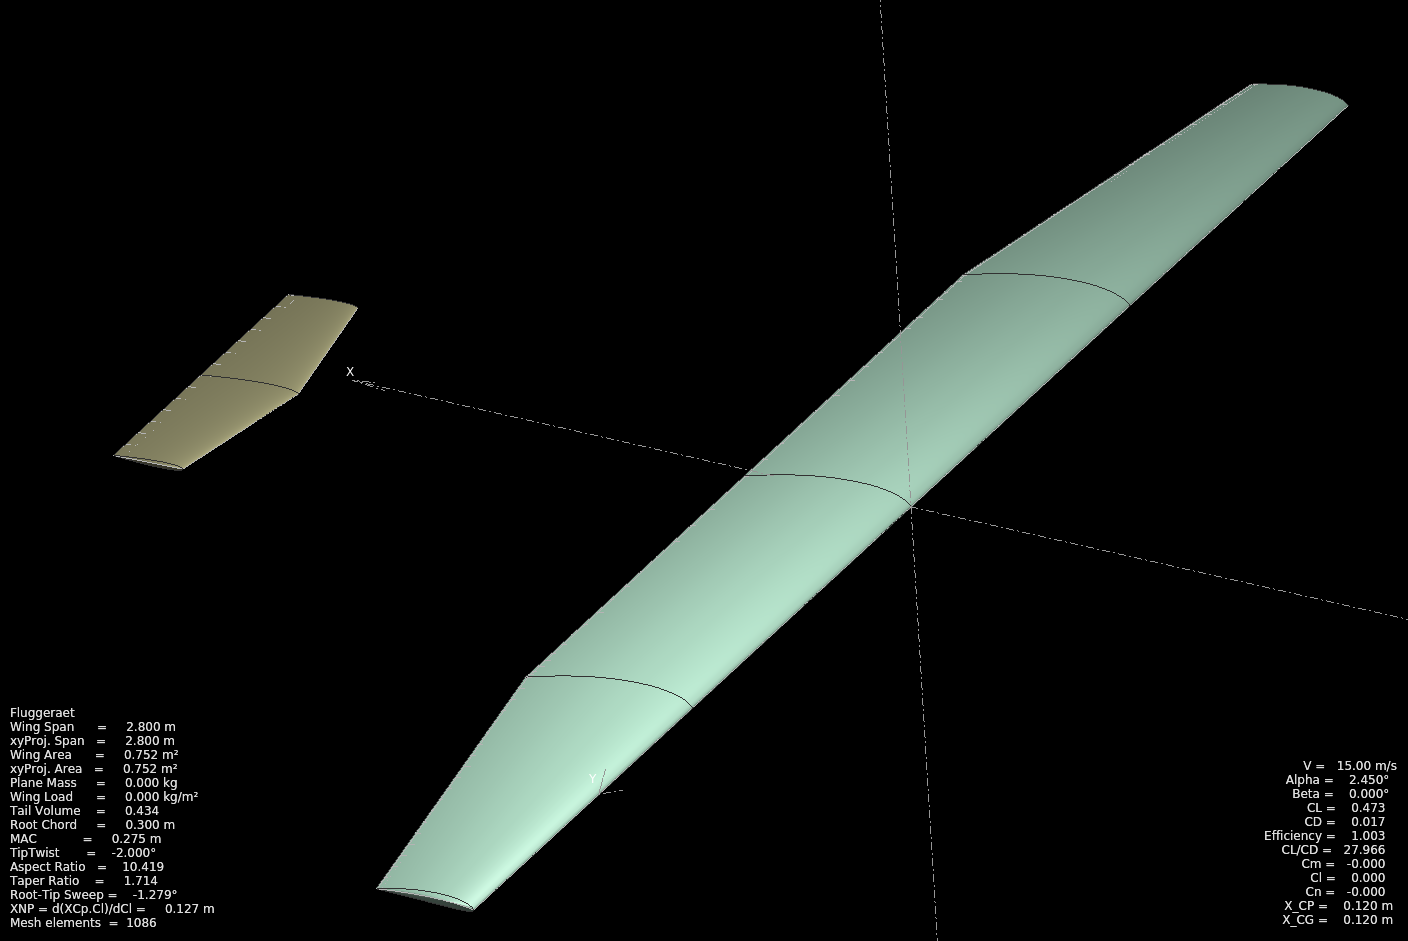
\includegraphics[width=0.9\textwidth]{bilder/Fotos/Aeroentwurf_Fluegelkonstruktion.png}
\caption{Stationärer Reiseflug bei 15 $m/s$ - entnommen den Berechnung in XFLR} 
\label{fig:Stationärer Reiseflug in XFLR}
\end{figure}

In diesem Fall ergibt die Ermittlung der aerodynamischen Beiwerte folgende Situation:

\begin{table}[h]
\centering
\begin{tabular}{|l|l|l|l|}
\hline
Parameter  & Bezeichnung &  Wert & Einheit \\ \hline
Fluggeschwindigkeit  & $V_{reise}$ & 15,00 & $m/s$\\ \hline
Abfluggewicht & $m_{reise}$  & 5,0 & $kg$\\ \hline
Anstellwinkel & $\alpha$ & 2,45 & $^\circ$ \\ \hline
Auftriebsbeiwert & $C_{L}$ & 0,473 & -\\ \hline
Widerstandsbeiwert & $C_{D}$ & 0,016  & -  \\ \hline
\end{tabular}
\caption{Errechnete Werte im stationären Reiseflug}
\label{tab:Errechnete Werte im Stationären Reiseflug}
\end{table}

In diesem Zustand ist der Flügel frei von Nickmomenten und das Höhenleitwerk erzeugt keine aerodynamischen Auftriebskräfte.

\clearpage

\subsection{Resultierende Kräfte und Momente}
\label{Resultierende Kräfte und Momenten Stationär}

In der stationären Flugsituation entstehen die folgenden maximalen Kräfte und Momente.

Biegemoment auf der 25\% Tiefenlinie der Tragfläche um die Einspannung in $Y = 0$
\begin{equation}
M_{b-X\,max} = 13,92 Nm    
\end{equation}

Drehmoment  um die 25\% Tiefenlinie an der Einspannung $Y = 0$
\begin{equation}
M_{t-Y\,max} \approx 0 Nm
\end{equation}
Für diesen Auslegungszustand ist der Schwerpunkt des Systems so gewähl, dass es im Arbeitspunkt nahezu momentenfrei fliegt. Das Höhenleitwerk kommt lediglich bei Abweichungen aus diesem Zustand zum Wirken.

\subsection{Kritische Lasten}

Gemäß CS 23.337 werden die positiven und negativen maximalen Manöverlastvielfachen berechnet.

Abflugmasse (take off weight) des Flugzeugs:
\begin{equation}
\label{eq:K1}
W_{0} = \SI{5}{\kilogram} = \SI{11,0231}{lb}
\end{equation}

Positive limit manoevering load factor:
\begin{equation}
\label{eq:K2}
n_{pos} = 2,1 + \frac{24000}{W_{0}+10000} = 4,4974 \qquad n_{pos gewählt}=4,5
\end{equation}

Negative limit manoevering load factor:
\begin{equation}
\label{eq:K3}
n_{neg} = (-0,4) \cdot n_{pos} = -1,7989 \qquad n_{neg_gewählt}=-1,8
\end{equation}

%/\begin{figure}[H]
%/\centering
%/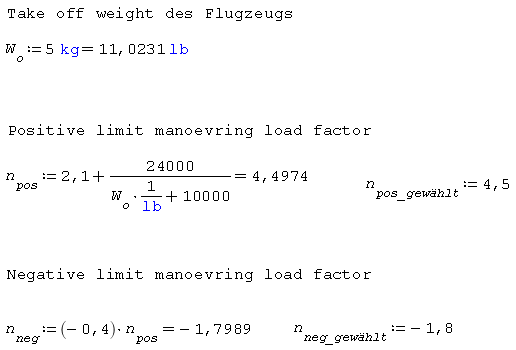
\includegraphics[width=0.9\textwidth]{bilder/Formeln/Kritische_Lastfaelle_Manoeverlasten.png}
%/\caption{Limit manoevring load factors nach CS23.337} 
%/\label{fig:Limit manoevring load factors nach CS23.337}
%/\end{figure}

%/Hochstart

%/Hier soll in konservativer Auslegung der Lasten für den gegebenfalls belastendensten Fall beim Hochstart mittels Gummiseil abgeschätzt werden. Hier übersteigt die Auftriebsbelastung für den Hochanstellwinkelbereich kurzeitig den Maximalauftrieb des Profils durch den Betrieb im instationären Bereich./%

%\\subsection{\colorbox{red}{Resultierende Kräfte und Momente}}
\label{Resultierende Kräfte und Momenten Kritisch}

\clearpage

\section{Betriebsgrenzen des Tragflügels}

Im Einsatz unterliegt das Tragwerk sowohl aerodynamischen als auch mechanischen Grenzen.
Diese werden Allgemein nach \cite{Sperl2011} berechnet.

Zunächst werden die kritischen Geschwindigkeiten für den Einsatz mit und ohne Klappen bestimmt:

\begin{equation}
\label{eq:K4}
c_{\text{L\ max\ Flap}} = 1.5 \qquad c_{\text{L\ max\ Clean}} = 1.3 
\end{equation}

\begin{equation}
\label{eq:K5}
V_{\text{S\,0}} = \sqrt{\cfrac{W_{0\ \text{MTOW}} \cdot \SI[per-mode = fraction]{9,81}{\meter\squared\per\second\squared}}{c_{\text{L\ max\ Flap}} \cdot \cfrac{\rho_{\text{Luft\ 0m}}}{2} \cdot S_{Wing}}}=\SI[per-mode = fraction]{8,42581}{\meter\per\second} \qquad V_{\text{S\,0\ gewählt}}=\SI[per-mode = fraction]{8,5}{\meter\per\second}
\end{equation}

\begin{equation}
\label{eq:K6}
V_{\text{stall\ gewählt}} = \sqrt{\cfrac{W_{0\ \text{MTOW}} \cdot \SI[per-mode = fraction]{9,81}{\meter\squared\per\second\squared}}{c_{\text{L\ max\ Clean}} \cdot \cfrac{\rho_{\text{Luft\ 0m}}}{2} \cdot S_{Wing}}}=\SI[per-mode = fraction]{9,05078}{\meter\per\second} \qquad V_{\text{stall\ gewählt}}=\SI[per-mode = fraction]{9,1}{\meter\per\second}
\end{equation}

%/\begin{figure}[H]
%/\centering
%/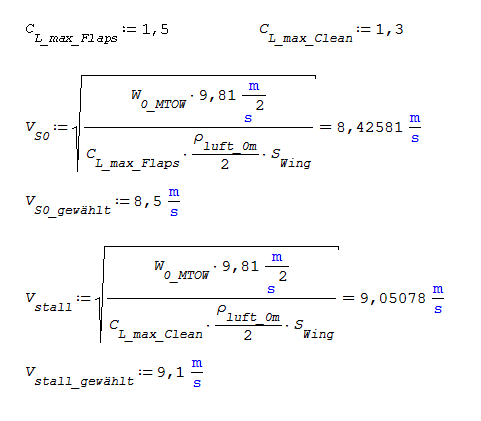
\includegraphics[width=0.9\textwidth]{bilder/Formeln/Mindestbetriebsgeschwindikeit.png}
%/\caption{Kritische Fluggeschwindikeiten} 
%/\label{fig:Kritische Fluggeschwindikeiten}
%/\end{figure}

Im selben Verfahren wird die Abrissgeschwindikeit (stall speed) für negative Werte des Auftriebs bestimmt:

\begin{equation}
\label{eq:K7}
c_{\text{L\ min\ Clean}} = 0.8 
\end{equation}
\begin{equation}
\label{eq:K8}
V_{\text{S\,neg}} = \sqrt{\cfrac{W_{0\ \text{MTOW}} \cdot \SI[per-mode = fraction]{9,81}{\meter\squared\per\second\squared}}{c_{\text{L\ min\ Clean}} \cdot \cfrac{\rho_{\text{Luft\ 0m}}}{2} \cdot S_{Wing}}}=\SI[per-mode = fraction]{11,53752}{\meter\per\second} \qquad V_{\text{S\,neg\ gewählt}}=\SI[per-mode = fraction]{11,6}{\meter\per\second}
\end{equation}

%/\begin{figure}[H]
%/\centering
%/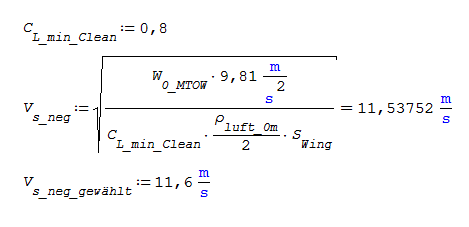
\includegraphics[width=0.9\textwidth]{bilder/Formeln/VS_neg.png}
%/\caption{Mindestgeschwindikeit für Invertierten Flug} 
%/\label{fig:Mindestgeschwindikeit für Invertierten Flug}
%/\end{figure}

Aus den Parametern ergibt sich im Weiteren die mindestens geforderte Höchstgeschwindigkeit beim Klappeneinsatz:

\begin{equation}
\label{eq:K8}
1.4 \cdot V_{\text{S\,0\ gewählt}}=\SI[per-mode = fraction]{11,9}{\meter\per\second} \quad
1.8 \cdot V_{\text{S\,0\ gewählt}}=\SI[per-mode = fraction]{16,38}{\meter\per\second} \quad
V_{\text{F\ gewählt}}=\SI[per-mode = fraction]{18}{\meter\per\second}
\end{equation}

%/\begin{figure}[H]
%/\centering
%/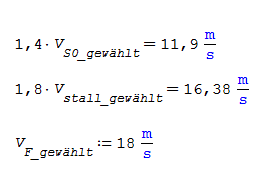
\includegraphics[width=0.9\textwidth]{bilder/Formeln/VF.png}
%/\caption{Klappenhöchstgeschwindigkeit} %/\label{fig:Klappenhöchstgeschwindigkeit}
%/\end{figure}

Des Weiteren ergeben sich die Manövergeschwindigkeiten $V_{A}$ und $V_{G}$ nach CS 23.335 zu:

\begin{equation}
\label{eq:K8}
V_{\text{A}}=V_{\text{S\,1\ gewählt}} \cdot \sqrt{n_{\text{pos}}}=\SI[per-mode = fraction]{19,304}{\meter\per\second} 
\end{equation}
\begin{equation}
\label{eq:K8}
V_{\text{G}}=V_{\text{S\,neg\ gewählt}} \cdot \sqrt{n_{\text{neg}}}=\SI[per-mode = fraction]{15,563}{\meter\per\second} 
\end{equation}

%/\begin{figure}[H]
%/\centering
%/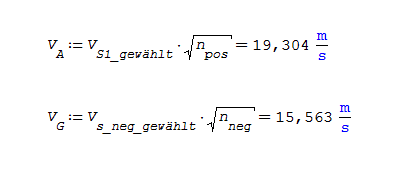
\includegraphics[width=0.9\textwidth]{bilder/Formeln/V_g.png}
%/\caption{Manövergeschwindigkeiten} 
%/\label{fig:Manövergeschwindigkeiten}
%/\end{figure}

\clearpage

Für den Dauerarbeitspunkt wird die Design Cruise Speed $V_{C}$ bestimmt:

\begin{equation}
\label{eq:K8}
W=\SI{11}{lb} \quad S=\SI{8,1}{ft^2}
\end{equation}
\begin{equation}
\label{eq:K8}
V_{\text{C\,min}}=33 \cdot \sqrt{\cfrac{W}{S}}=\SI{38,4563}{kn}=\SI[per-mode = fraction]{19,7804}{\meter\per\second}
\end{equation}
Berechnung von $V_{\text{C\,max}}$ entfällt mangels einer Leistungsauslegung
\begin{equation}
\label{eq:K8}
V_{\text{C\ gewählt}}=\SI[per-mode = fraction]{20}{\meter\per\second} 
\end{equation}

%/\begin{figure}[H]
%/\centering
%/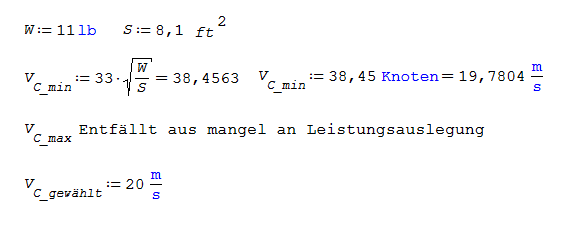
\includegraphics[width=0.9\textwidth]{bilder/Formeln/V_c.png}
%/\caption{Design Cruise Speed} 
%/\label{fig:Design Cruise Speed}
%/\end{figure}

Aus dieser lässt sich die maximal nicht zu überschreitende Geschwindigkeit $V_{D}$ ableiten:

\begin{equation}
\label{eq:K8}
V_{\text{D\,min\,1}}=1.25 \cdot V_{\text{C\,max}} \quad 
\end{equation}
Berechnung von $V_{\text{D\,min\,1}}$ entfällt mangels $V_{\text{C\,max}}$
\begin{equation}
\label{eq:K8}
V_{\text{D\,min\,2}}=1.35 \cdot V_{\text{C\ gewählt}}=\SI[per-mode = fraction]{27}{\meter\per\second} 
\end{equation}

%/\begin{figure}[H]
%/\centering
%/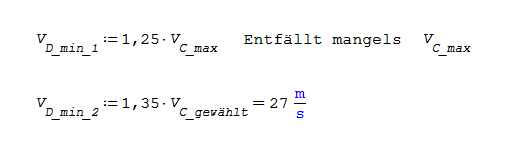
\includegraphics[width=0.9\textwidth]{bilder/Formeln/V_d.png}
%/\caption{Maximale Sturzgeschwindikeit} 
%/\label{fig:Maximale Sturzgeschwindikeit}
%/\end{figure}

\begin{landscape}
\begin{figure}[H]
\centering
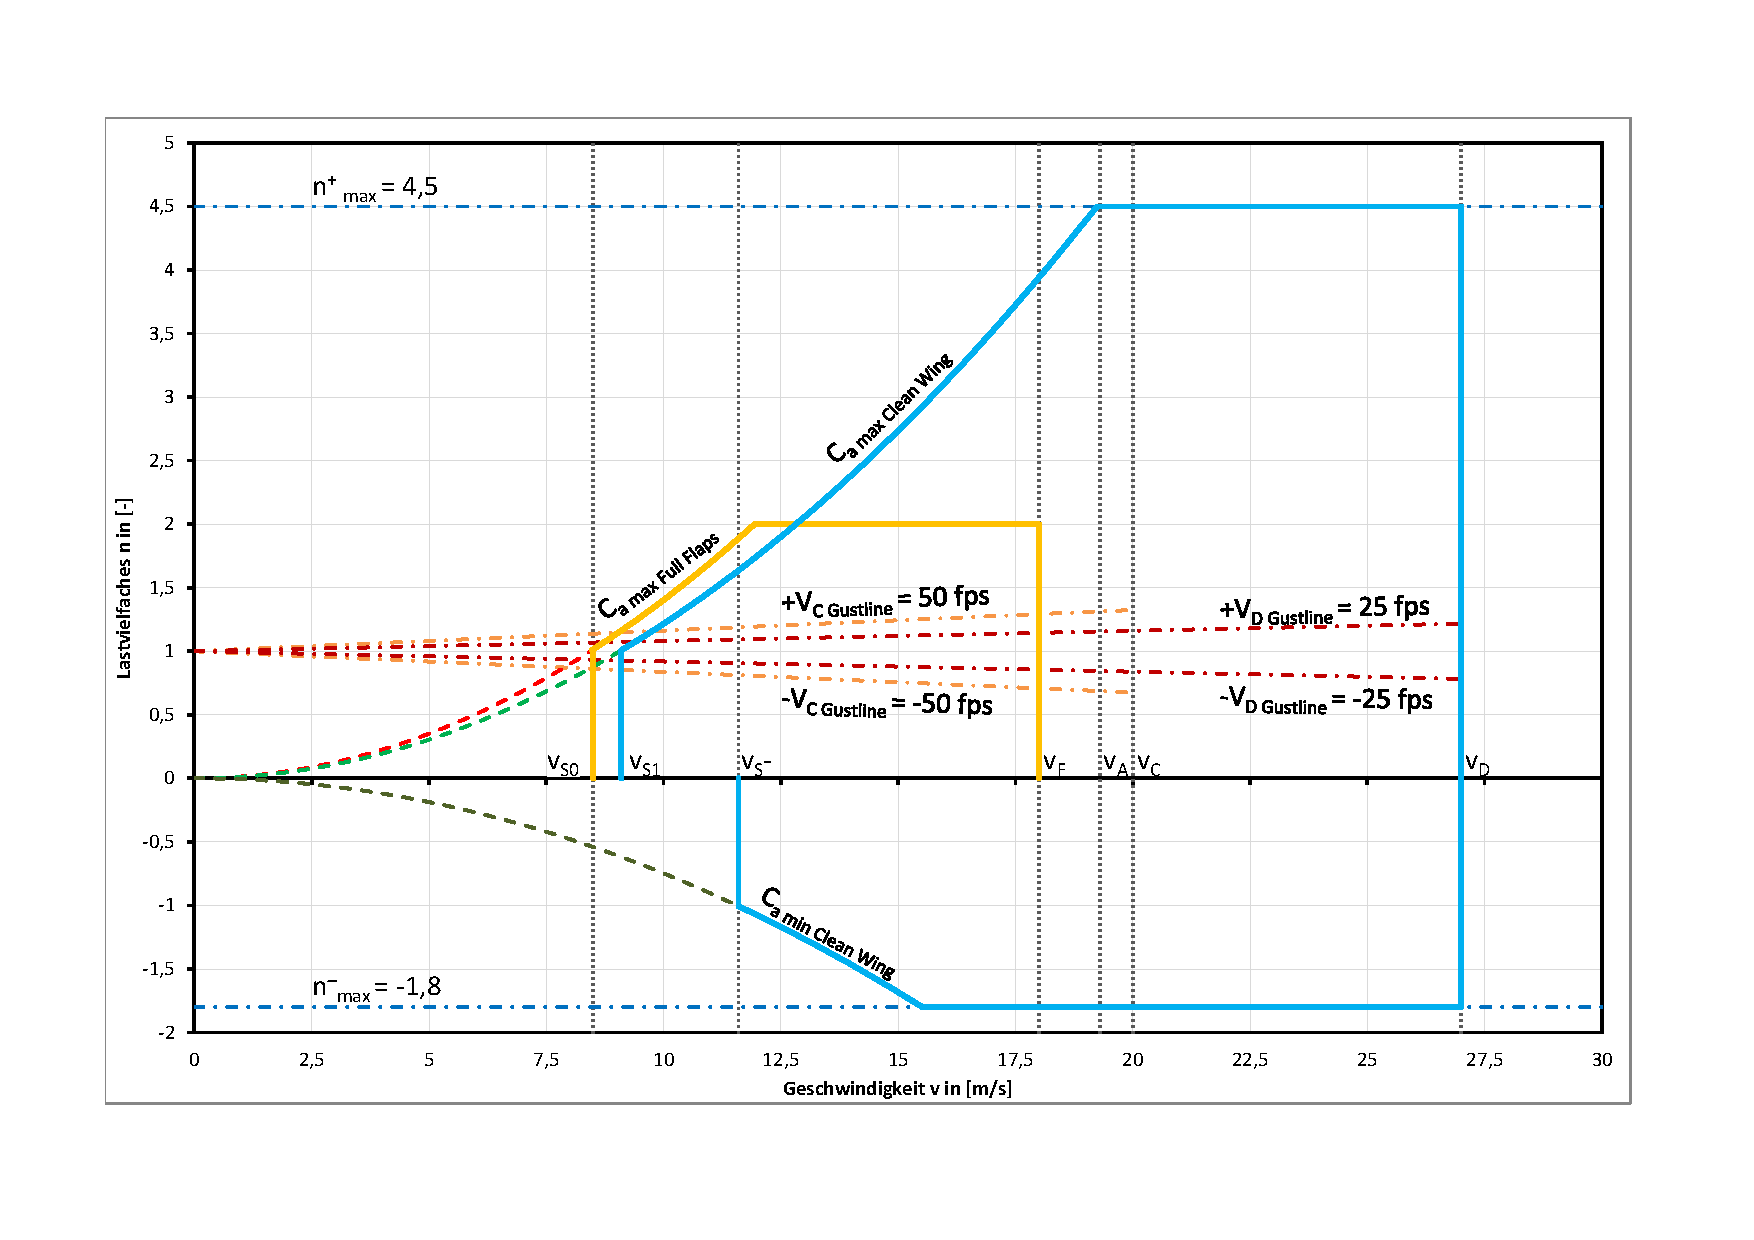
\includegraphics[height=0.945\textheight, trim={20mm 24mm 22mm 22mm},clip]{bilder/Formeln/VN-Diaggramm-rev-00.pdf}
\caption{Betriebsbereich im V\textsubscript{n}-Diagramm} 
\label{fig:Vn Diagramm des Flugsystems}
\end{figure}
\end{landscape}